% {{{
\documentclass[12pt]{article}
\usepackage[tmargin=0.75in,bmargin=0.75in,lmargin=0.9in,rmargin=0.9in]{geometry}

\usepackage{amsmath}
\include{latexsym}
\include{amssymb}
\usepackage{enumitem}
\usepackage[symbol, hang]{footmisc}
\usepackage{indentfirst}
\usepackage{amssymb}
\usepackage{graphicx,psfrag}

\def\F{\mathcal{F}}
\def\M{\mathcal{M}}
\def\dimspec{\mathfrak{D}}
\def\htop{h_{top}}
\def\trans{\mathcal{T}}
\def\G{\mathcal{G}}
\newcommand{\Z}{\mathbb{Z}}
\pagenumbering{gobble}
\def\O{\mathcal{O}}

\newcommand\NoIndent[1]{%
  \begingroup
  \par
  \parshape0
  #1\par
  \endgroup
}
% }}}

% Title {{{
\begin{document}

\begin{center}
{\large \bf CompMethods }   \\ \large pset4 \\ Ephraim Sutherland
\end{center}
% }}}

% \subsection*{Problems}

\begin{enumerate}

	\item First, in figure $a$, we can see that the path of capital converges to a steady state that is just below 3.0. 
		\\\\  We can also see that for $T=41$,  $\sum_{t=0}^{T}\beta^t U(c_t) = 3.235163626817102 $
		and $\bar v_i = 3.2683299286113185$ Where our initial  $i$ is simply $i = N = 31$.
		Thus the  difference $ | \bar v_i - \sum_{t=0}^{T}\beta^t U(c_t) | = | 3.2683299286113185 - 3.235163626817102 | \approx 0.03316630179421676$ Thus it is quite small and seems to have converged.
		\begin{center}
			\textbf{a}\par\medskip
			\includegraphics[width=0.8\linewidth]{plot_k1.png}
			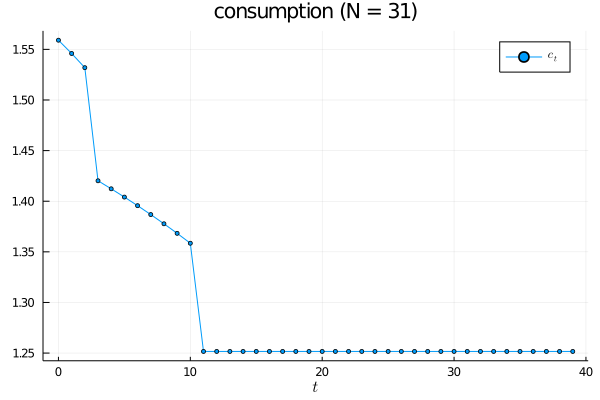
\includegraphics[width=0.8\linewidth]{plot_c.png}
		\end{center}
	\item 
		Value function iteration converged in 111 iterations (maxerr = 9.171100527893827e-7)
		\\
		--------------------------------------------------------------------------------
		\\ Problem 2 - minimization \\
		--------------------------------------------------------------------------------
		\\\\
		----------------------------------------
		\\using brent's method: \\
		----------------------------------------
		\\\\
		Function max obtained at 1.0000 with function value -1.0. converged after 13 iterations \\
		\\ ---------------------------------------- \\
		\\     using Newton-Raphson method:   \\
		\\ ---------------------------------------- \\
		\\  \\
		\\ Function max obtained at 1.0000 with function value -1.0. converged after 16 iterations \\
		\\  \\
	\item 
		-------------------------------------------------------------------------------- \\
		\\     Problem 3 - minimization  \\
		\\ -------------------------------------------------------------------------------- \\
		\\ 
		\\ ---------------------------------------- \\
		\\     using Newton-Raphson method:   \\
		\\ ---------------------------------------- \\
		\\  \\
		\\ Function min obtained at [6.931471805599456, 6.931471805599456] with function value 3.944304526105059e-31. converged after 7 iterations \\
		\\  \\
\end{enumerate} 

\end{document}


